\clearpage\subsection*{教材を自分のフォルダに置こう}
まずは、今回利用する教材をコピーしましょう。
これまでと同じように、/usr/local/share/ome という場所にあるフォルダ 07をコピーして、/home/ユーザー名 に貼り付けてください。

やり方を忘れてしまった人は、「第1回 4.1 例題1-18 教材をじぶんのフォルダに置こう」 を参考にしてみてください。

\subsection*{1−1インターネットのキホン}
\refstepcounter{PagePtr}\label{P:internet}
\begin{wrapfigure}{r}[10pt]{0.4\textwidth}
	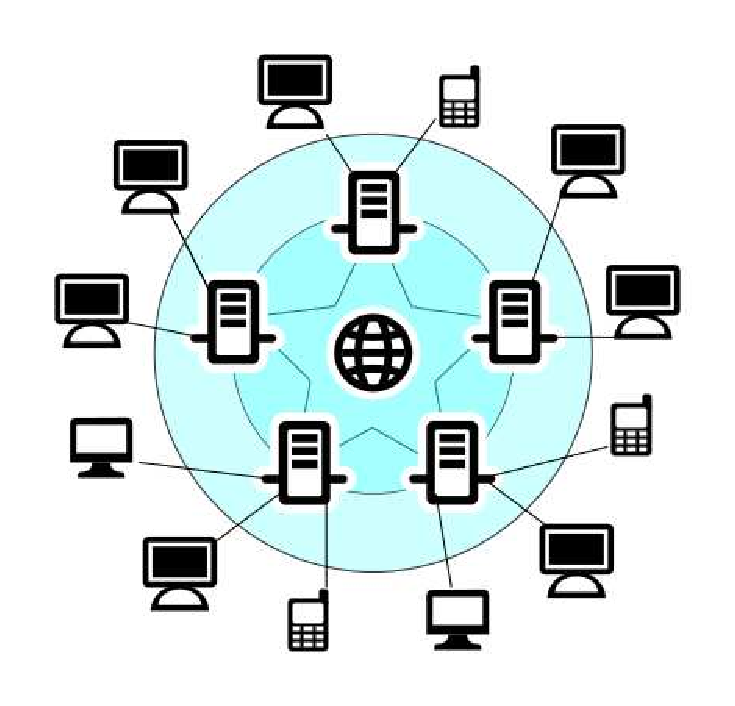
\includegraphics[width=0.4\textwidth]{ome7-img002.eps}
\end{wrapfigure}

みんなが使っているパソコンやスマートフォンなどをたくさんつなぎ、おたがいに情報の\ruby{交換}{こうかん}ができるようにしたものを「ネットワーク」とよんでいます。

インターネットとは、そのネットワークが数えきれないほどのケーブルなどでおたがいにつながりあい、\ruby{網}{あみ}の目のように世界中に広がっているそのもののことです。


\bigskip

みなさんはすでにインターネットを\ruby{触}{さわ}っています。

第一回の\ruby{講義}{こうぎ}でみなさんはwebから画像を自分のラズベリーパイ(PC)に保存しましたね。あれもインターネットを触ったということになるのです。網目のように世界中に広がっているネットワークから好きな画像を調べるということは自分のラズベリーパイでインターネットをしたということになります。

さらに、有名な動画サイト”YouTube”のコンピュータもインターネットにつながっています。そのおかげでインターネットにつながっているパソコンやスマートフォンであればYouTubeの動画を見ることができます。もちろん、インターネットにつながっていなければYouTubeの動画や画像\ruby{検索}{けんさく}など行うことはできません。試しにインターネットを\ruby{切断}{せつだん}してみても面白いかもしれません。


\vfill

\refstepcounter{Question}\theQuestion みんなが使っているパソコンやスマートフォンなどをたくさんつなぎ、おたがいに情報の交換ができるようにしたものを何というでしょうか。\label{Q:internet}




\bigskip

\bigskip

\bigskip

\addBlank{答え}


\bigskip


\bigskip


\bigskip


\bigskip


\clearpage

\subsection*{ 1−2 IPアドレスとは何だろう?}
\refstepcounter{PagePtr}\label{P:IP}

ネットワークでコンピュータ同士がつながっているときにどうやって通信相手のコンピュータの場所を\ruby{探}{さが}すのでしょうか?

わたしたちのいる住んでいる場所をしめす住所(英語でアドレス)と同じ考え方を使います。
インターネットの住所のことをIP(アイピー)アドレスと言います。
わたしたち日本人は住所を東京都港区高輪2−3−23(東海大学高輪キャンパスの住所)のように表します。
コンピュータの場合は\textbf{数字}で表します。
IPアドレスの場合はxxx.xxx.xxx.xxxのように四つの数字を使って表します。
3ケタづつ「\textbf{.}」点(ドット)で区切ります。
xxxは0~255の数字が入ります。


\bigskip


\centering
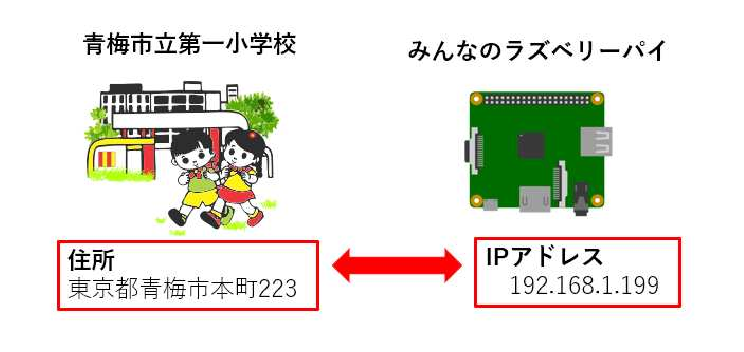
\includegraphics[width=0.8\textwidth]{ome7-img003}


\bigskip


\bigskip


\bigskip





\centering
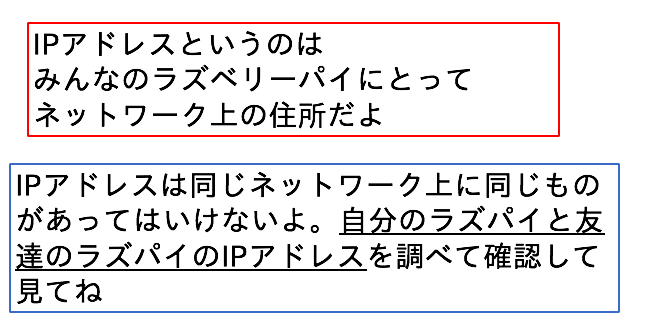
\includegraphics[width=0.8\textwidth]{ome7-img004.png}
\flushleft


\bigskip


\bigskip


\bigskip


\bigskip


\bigskip

IPアドレスはラズベリーパイのネットワーク上の住所に当たるものです。一つのネットワークではIPアドレスは同じものがあってはいけません。例えば、配達する人は同じ住所が世界中にあればどこへ配達したらよいかわからなくなってしまいます。インターネットの場合も同じです。なのでIPアドレスは同じではいけません。ですが、例外として他のローカルIPアドレスでは同じになってしまうことはあります。%\textbf{例題7−1で自分のラズベリーパイのIPアドレスを調べましょう}

\clearpage\subsection*{\bfseries
	1−3 グローバルIPアドレスとローカルIPアドレス}
IPアドレスにはグローバルIPアドレスとローカル(プライベート)IPアドレスという二つに分けられます。



\centering
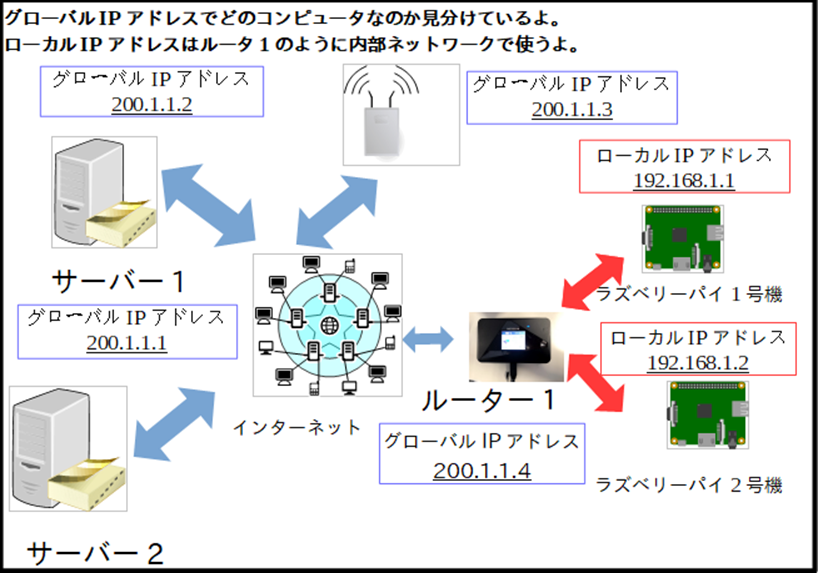
\includegraphics[width=15.0cm]{ome7-img005.png}

\centering
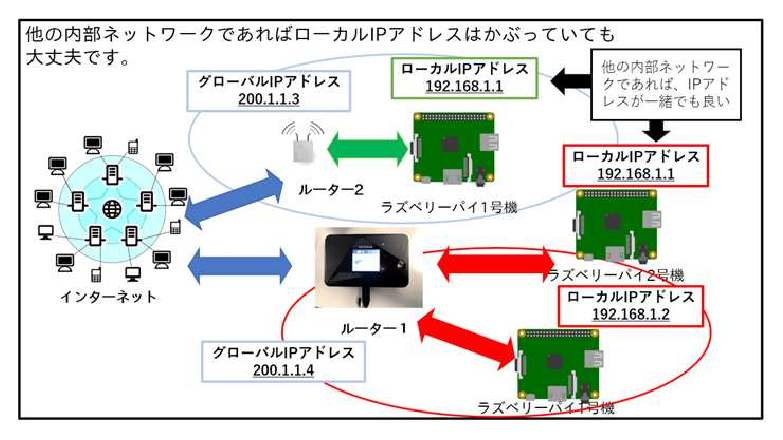
\includegraphics[width=15.0cm]{ome7-img006}
\flushleft

{\refstepcounter{Question}\theQuestion ローカルIPアドレスがかぶっても良いときはどのときですか。\label{Q:localIP}}

{\bfseries
	\addBlank{答え}}

	\refstepcounter{Exercise}
\clearpage\subsection*{\theExercise IPアドレスを調べてみよう\label{E:checkIP}}
ターミナルにコマンド”hostname
-\texttt{I}”を入力し、自分のラズベリーパイのローカルIPアドレスを確認しよう

{\bfseries
方法}



\centering
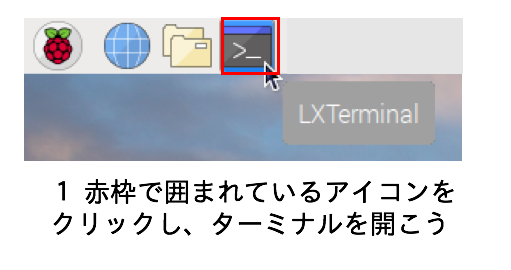
\includegraphics[width=0.85\textwidth]{ome7-img007.png}

\centering
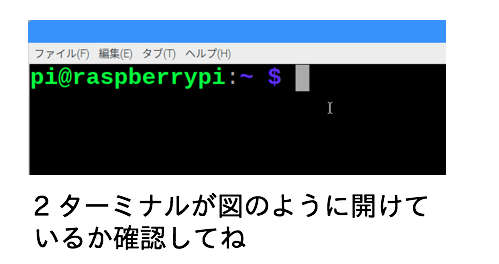
\includegraphics[width=0.85\textwidth]{ome7-img008.png}
\flushleft

\clearpage

\centering

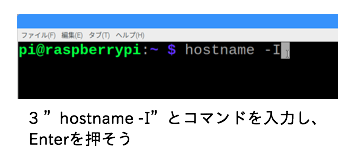
\includegraphics[width=0.85\textwidth]{ome7-img010.png}
\centering
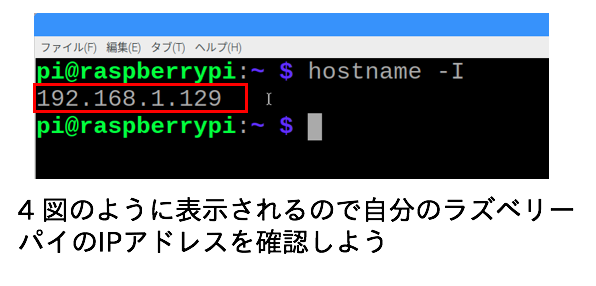
\includegraphics[width=0.85\textwidth]{ome7-img009.png}
\flushleft


\bigskip


\bigskip


\bigskip


\bigskip

{\bfseries
	調べた自分のラズベリーパイのIPアドレスを書こう}

\bigskip


\centering
\begin{tabular}{|p{0.8\textwidth}|} \hline
	\\
	\\
	\\
	\\ \hline
\end{tabular}


\bigskip


\bigskip

\flushleft

{\bfseries
	グループの友達のIPアドレスも教えてもらって書こう}

\bigskip


\centering
\begin{tabular}{|p{0.8\textwidth}|} \hline
	\\
	\\
	\\
	\\ \hline
\end{tabular}


\flushleft


